% !TEX TS-program = pdflatex
% !TEX encoding = UTF-8 Unicode

\documentclass[a4paper, titlepage=false, parskip=full-, 10pt]{scrartcl}

\usepackage[utf8]{inputenc}
\usepackage[T1]{fontenc}
\usepackage[english, ngerman]{babel}
\usepackage{babelbib}
\usepackage{hyperref}
\usepackage{listings}
\usepackage{framed}
\usepackage{color}
\usepackage{graphicx}
\usepackage[normalem]{ulem}
\usepackage{cancel}
\usepackage{amsmath}
\usepackage{amssymb}
\usepackage{amsthm}
\usepackage{algorithm}
\usepackage{algorithmic}
\usepackage{geometry}
\usepackage{subfigure}
\geometry{a4paper, top=20mm, left=35mm, right=25mm, bottom=40mm}

\newcounter{tasknbr}
\setcounter{tasknbr}{1}
\newenvironment{task}[1]{{\bf Aufgabe \arabic {tasknbr}\stepcounter{tasknbr}} (#1):\begin{enumerate}}{\end{enumerate}}
\newcommand{\subtask}[1]{\item[#1)]}

% Listings -----------------------------------------------------------------------------
\definecolor{red}{rgb}{.8,.1,.2}
\definecolor{blue}{rgb}{.2,.3,.7}
\definecolor{lightyellow}{rgb}{1.,1.,.97}
\definecolor{gray}{rgb}{.7,.7,.7}
\definecolor{darkgreen}{rgb}{0,.5,.1}
\definecolor{darkyellow}{rgb}{1.,.7,.3}
\lstloadlanguages{C++,[Objective]C,Java}
\lstset{
escapeinside={§§}{§§},
basicstyle=\ttfamily\footnotesize\mdseries,
columns=fullflexible,
keywordstyle=\bfseries\color{blue},
commentstyle=\color{darkgreen},      
stringstyle=\color{red},
numbers=left,
numberstyle=\ttfamily\scriptsize\color{gray},
breaklines=true,
showstringspaces=false,
tabsize=4,
captionpos=b,
float=htb,
frame=tb,
frameshape={RYR}{y}{y}{RYR},
rulecolor=\color{black},
xleftmargin=15pt,
xrightmargin=4pt,
aboveskip=\bigskipamount,
belowskip=\bigskipamount,
backgroundcolor=\color{lightyellow},
extendedchars=true,
belowcaptionskip=15pt}

%% Enter current values here: %%
\newcommand{\lecture}{Computer Vision WS15/16}
\newcommand{\tutor}{}
\newcommand{\assignmentnbr}{4}
\newcommand{\students}{Julius Auer}
%%-------------------------------------%%

\begin{document}  
{\small \textsl{\lecture \hfill \tutor}}
\hrule
\begin{center}
\textbf{Übungsblatt \assignmentnbr}\\
[\bigskipamount]
{\small \students}
\end{center}
\hrule

\begin{task}{CAMSHIFT (Teil 2)}
\item[]\emph{\begin{itemize}
\item implementiere die Berechnung des Fensterzentrums, -größe und Objektorientierung wie im Paper
\item tracke das Auto vom ersten zum letzten Frame
\end{itemize}}

Nun, ich hatte die Aufgabe ja aus Versehen letzte Woche schon gelöst. Um nicht ganz untätig zu sein, habe ich diese Woche meine Lösung nach C++ portiert, um sie Echtzeit-fähig zu machen (der Octave-Prototyp von letzter Woche war zu langsam, um das ganze Video zu verarbeiten).

Das Ergebnis ist sehr gut. Für Basis-Operationen wie Farbraum-Konvertierungen und IO benutze ich OpenCV, CAMShift selbst ist von mir implementiert (obwohl OpenCV das auch angeboten hätte). Ich habe den Code und das Ergebnis als Video hochgeladen. Einzelbilder zeigt Abbildung \ref{fig:1-1}.

Was die eigentliche Aufgabenstellung betrifft, wiederhole ich nur kurz das Wesentliche vom letzten Zettel:

\begin{itemize}
\item Da hier kein Fleisch sondern ein Auto getrackt wird, muss an einigen Stellen vom Vorgehen im Paper abgewichen werden:
\item Für das Hue-Bild wird ein Fehler anhand der Satuation-Werte berechnet (bei Fleisch: Value)
\item Die Aspect-Ratio für das neue Fenster wird aus $M_{20},M_{02}$ berechnet (bei Fleisch: fest)
\item Der Roll des Kopfes wird nicht berechnet (es gibt keinen Kopf)
\item Details zu diesen Anpassungen (mit Bildern) finden sich auf meinem letzten Übungszettel
\end{itemize}

\begin{figure}[!htpb]
\centering
\subfigure[Frame 1]{
  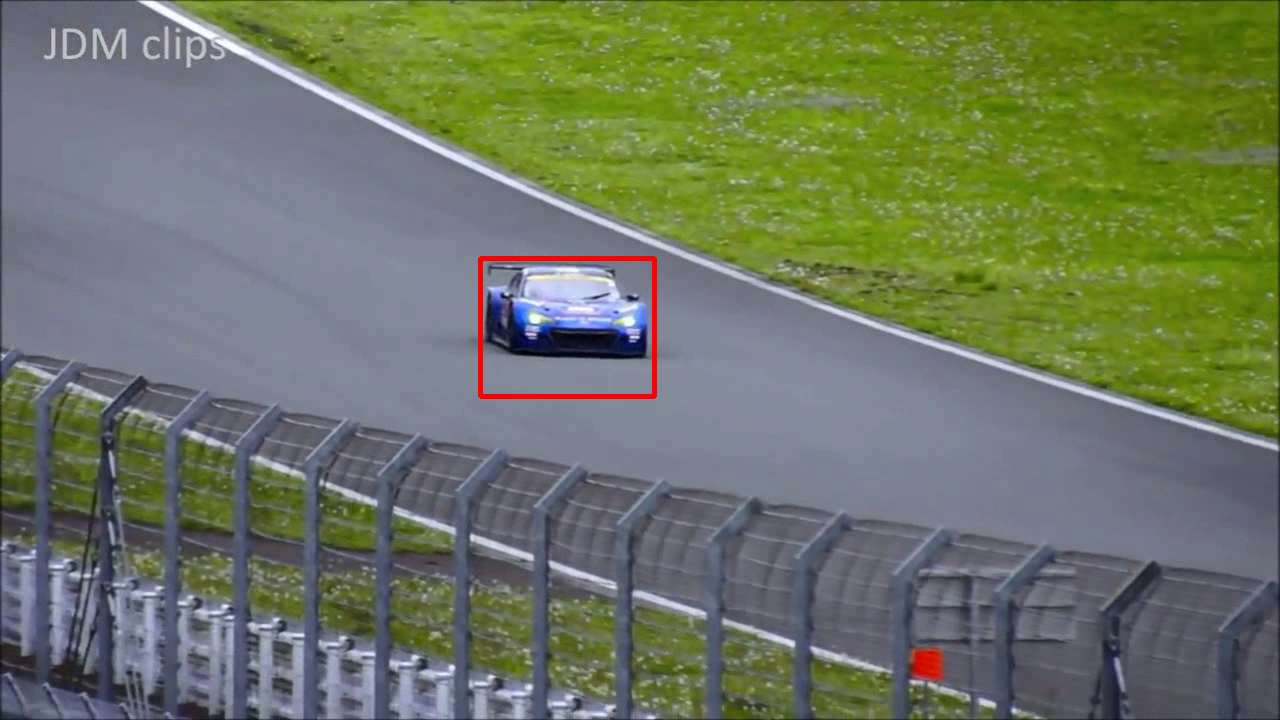
\includegraphics[width=0.48\linewidth]{captures/capture_1-1}
}
\subfigure[Frame 50]{
  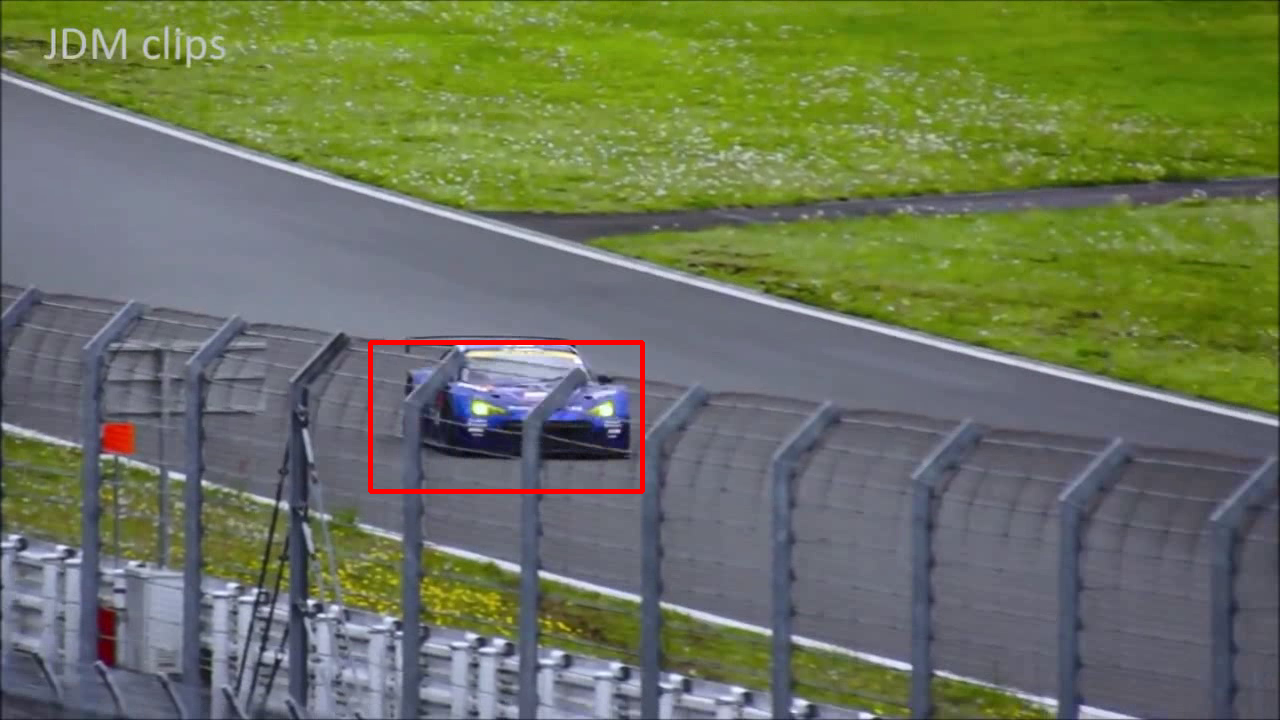
\includegraphics[width=0.48\linewidth]{captures/capture_1-2}
}
\subfigure[Frame 100]{
  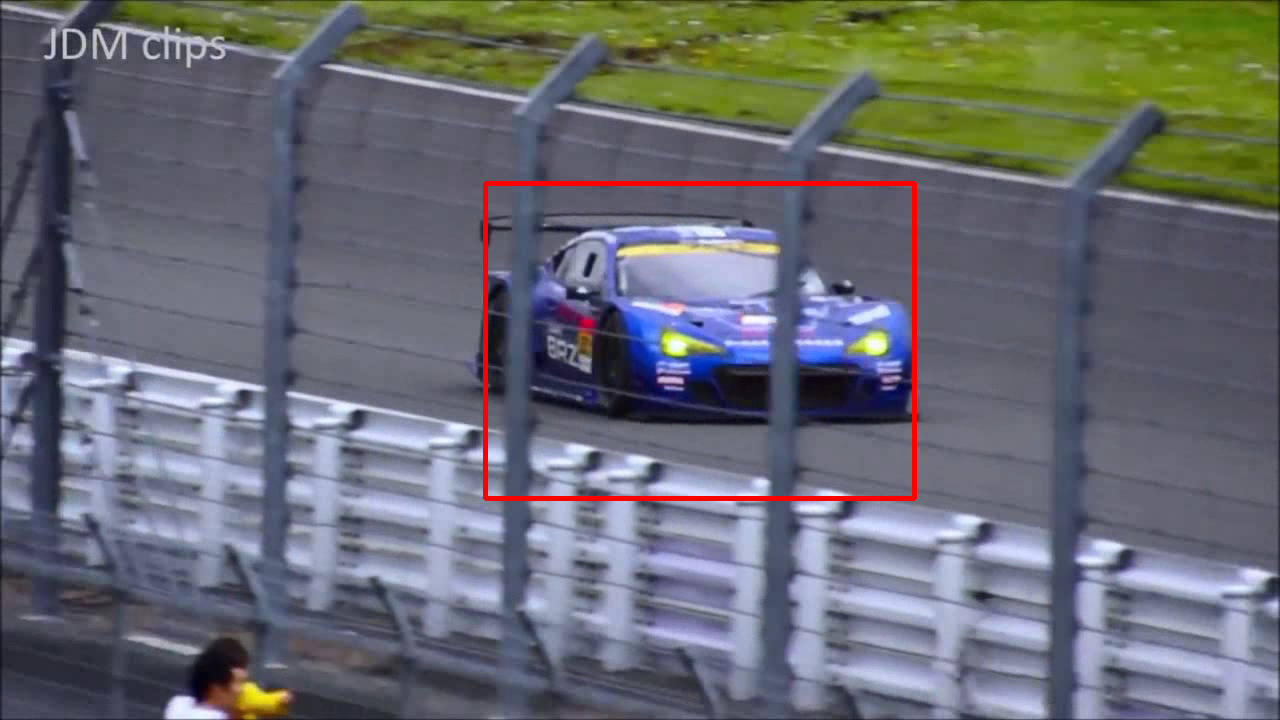
\includegraphics[width=0.48\linewidth]{captures/capture_1-3}
}
\subfigure[Frame 200]{
  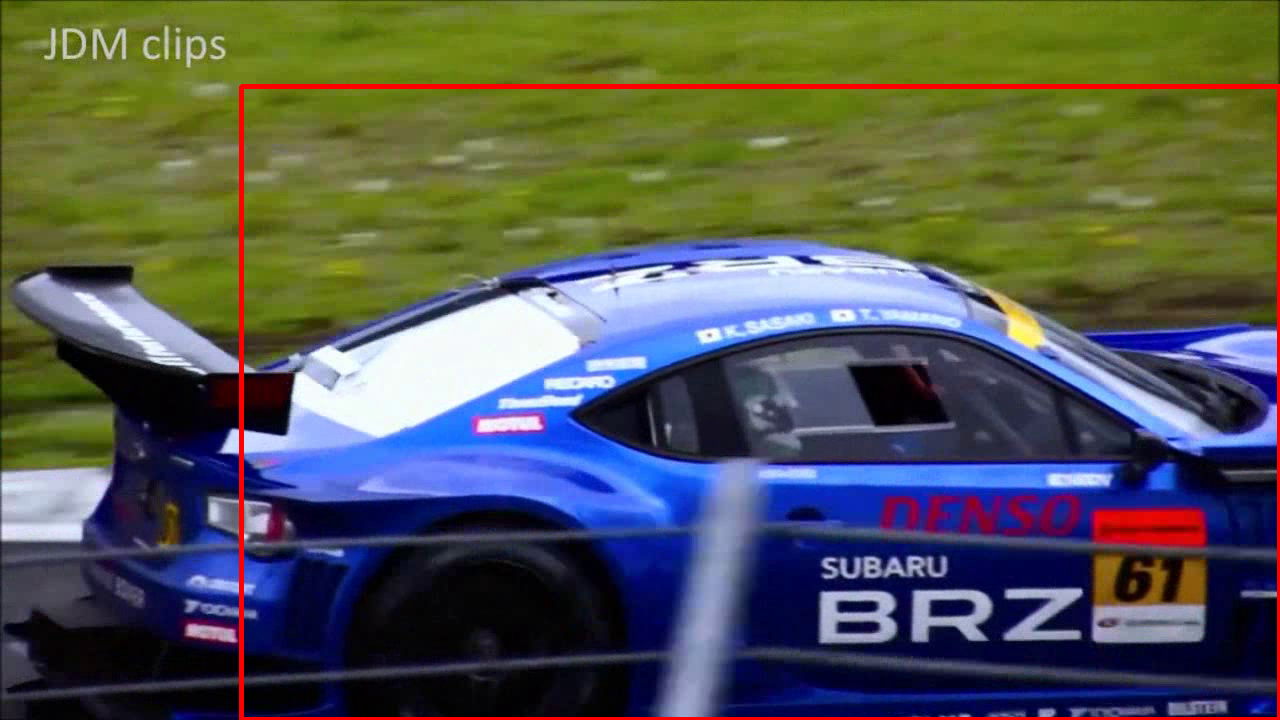
\includegraphics[width=0.48\linewidth]{captures/capture_1-4}
}
\subfigure[Frame 250]{
  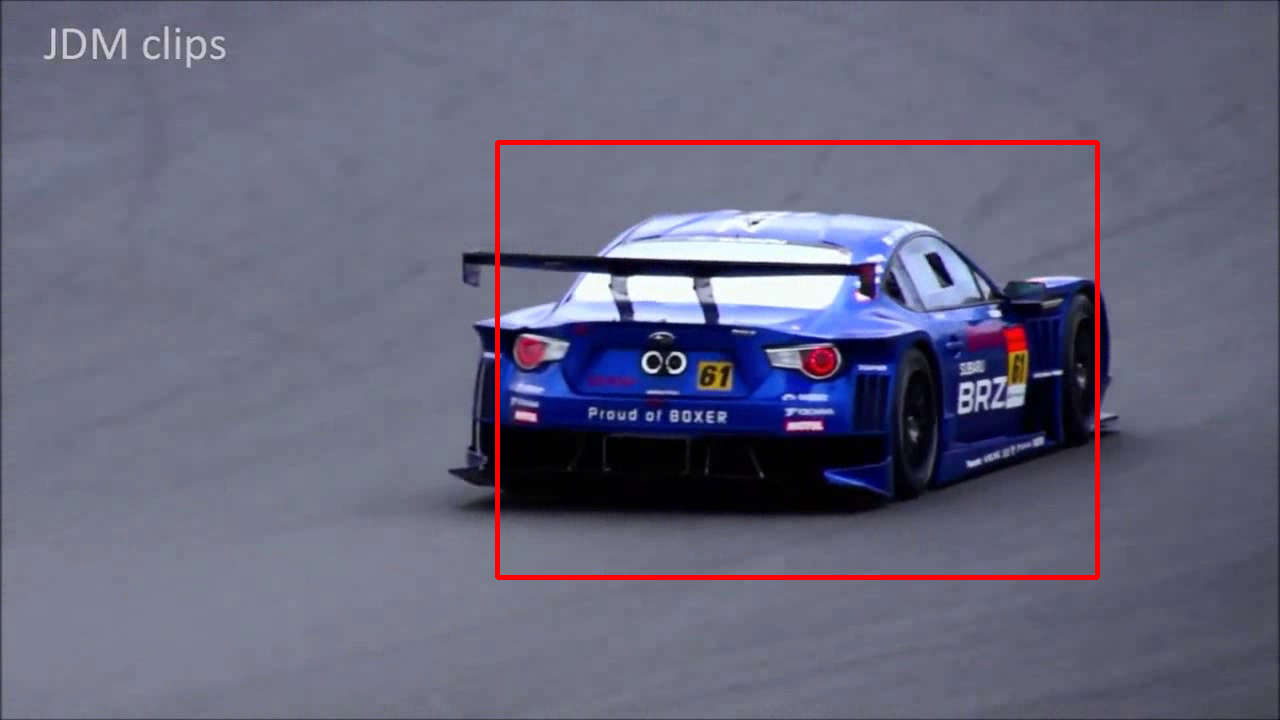
\includegraphics[width=0.48\linewidth]{captures/capture_1-5}
}
\subfigure[Frame 300]{
  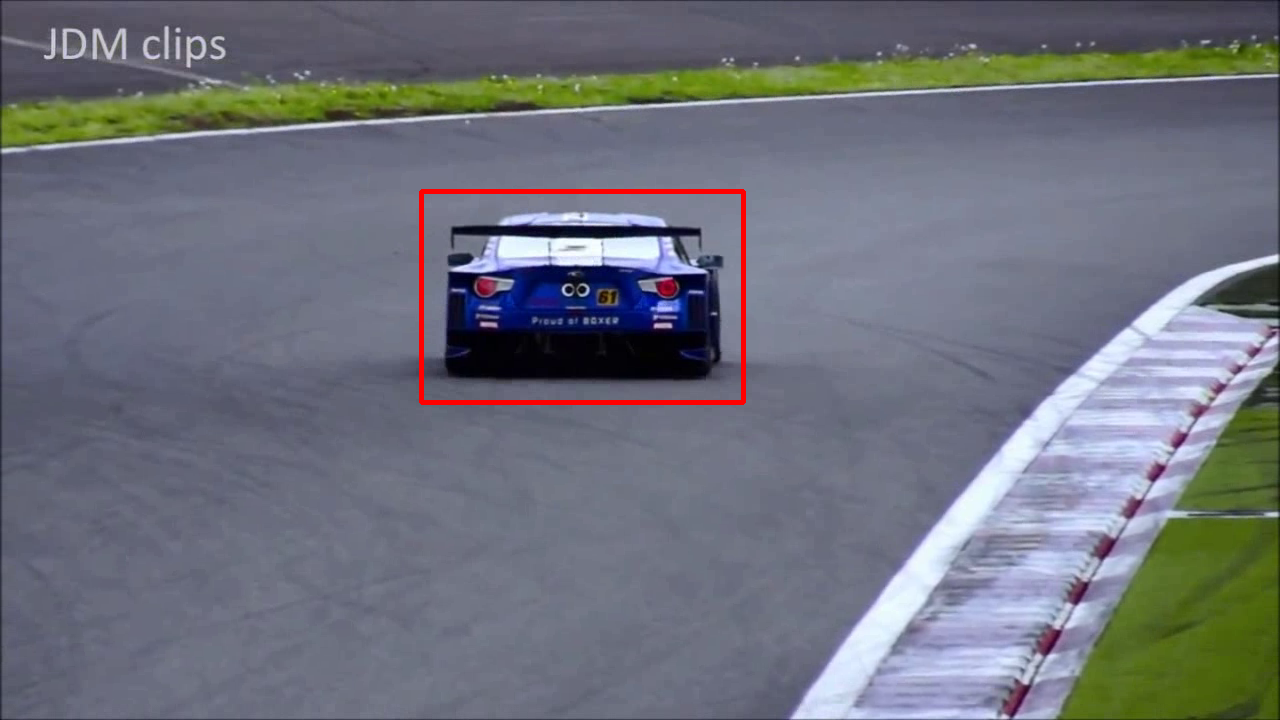
\includegraphics[width=0.48\linewidth]{captures/capture_1-6}
}
\caption{Resultat (Auszug)}
\label{fig:1-1}
\end{figure}
\end{task}

\newpage
\begin{task}{Hu-Momente}
\item[]\emph{\begin{itemize}
\item lies das paper:\\
\url{http://www.sci.utah.edu/~gerig/CS7960-S2010/handouts/Hu.pdf}\\
\item implementiere die sieben Momente von Hu
\item nimm an, wir suchen ein Symbol ('needle.png') in einem Bild voller Symbole ('haystack.png')
\item berechne die sieben Momente für das gesuchte Symbol
\item suche die bounding boxes der Symbole im Haystack (wenn ihr mögt auch gerne über Drittsoftware)
\item bestimme für jedes Symbol im Haystack die Ähnlichkeit (oder den Abstand) seiner sieben Momente zu denen des gesuchten Symbols
\end{itemize}}

Dazu habe ich nur wenig zu sagen: Der Code ist C++ (wieder mit ein bisschen OpenCV) wobei ich - aus purer Lust am Coden - {\bf nicht} von OpenCV die Bildmomente habe berechnen lassen, sondern alle $M,\mu,I$ selbst ausrechne. Das ist der schrecklichste, unleserlichste Code den ich seit langem geschrieben habe :D

Ich lasse von OpenCV die Bounding-Boxes berechnen (Abbildung \ref{fig:2-1}), berechne dann für \emph{Needle} und alle Boxen jeweils alle Hu-Momente und betrachte den Quadratischen Fehler. Die Box mit dem geringsten Fehler beinhaltet erwartungsgemäß die Nadel (Abbildung \ref{fig:2-2}).

\begin{figure}[!htpb]
\centering
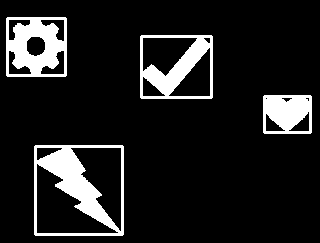
\includegraphics[width=0.7\linewidth]{captures/capture_2-1}
\caption{Alle Bounding-Boxes (von OpenCV berechnet)}
\label{fig:2-1}
\end{figure}

\begin{figure}[!htpb]
\centering

\includegraphics[width=0.7\linewidth]{captures/capture_2-2}
\caption{Die Box mit dem niedrigsten Fehler}
\label{fig:2-2}
\end{figure}
\end{task}
\end{document}